\documentclass[reqno,11pt]{amsart}
\usepackage{epsfig,amscd,amssymb,amsmath,amsfonts}
\usepackage{amsmath}
\usepackage{amsthm,color}
\usepackage{tikz}
\usetikzlibrary{graphs}
\usetikzlibrary{graphs,quotes}
\usetikzlibrary{decorations.pathmorphing}
\tikzset{snake it/.style={decorate, decoration=snake}}
\tikzset{snake it/.style={decorate, decoration=snake}}
\usetikzlibrary{decorations.pathreplacing,decorations.markings,snakes}
\usepackage[colorlinks]{hyperref}
\usetikzlibrary{graphs}
\usetikzlibrary{graphs,quotes}
\usetikzlibrary{decorations.pathmorphing}
\tikzset{snake it/.style={decorate, decoration=snake}}
\tikzset{snake it/.style={decorate, decoration=snake}}

\begin{document}

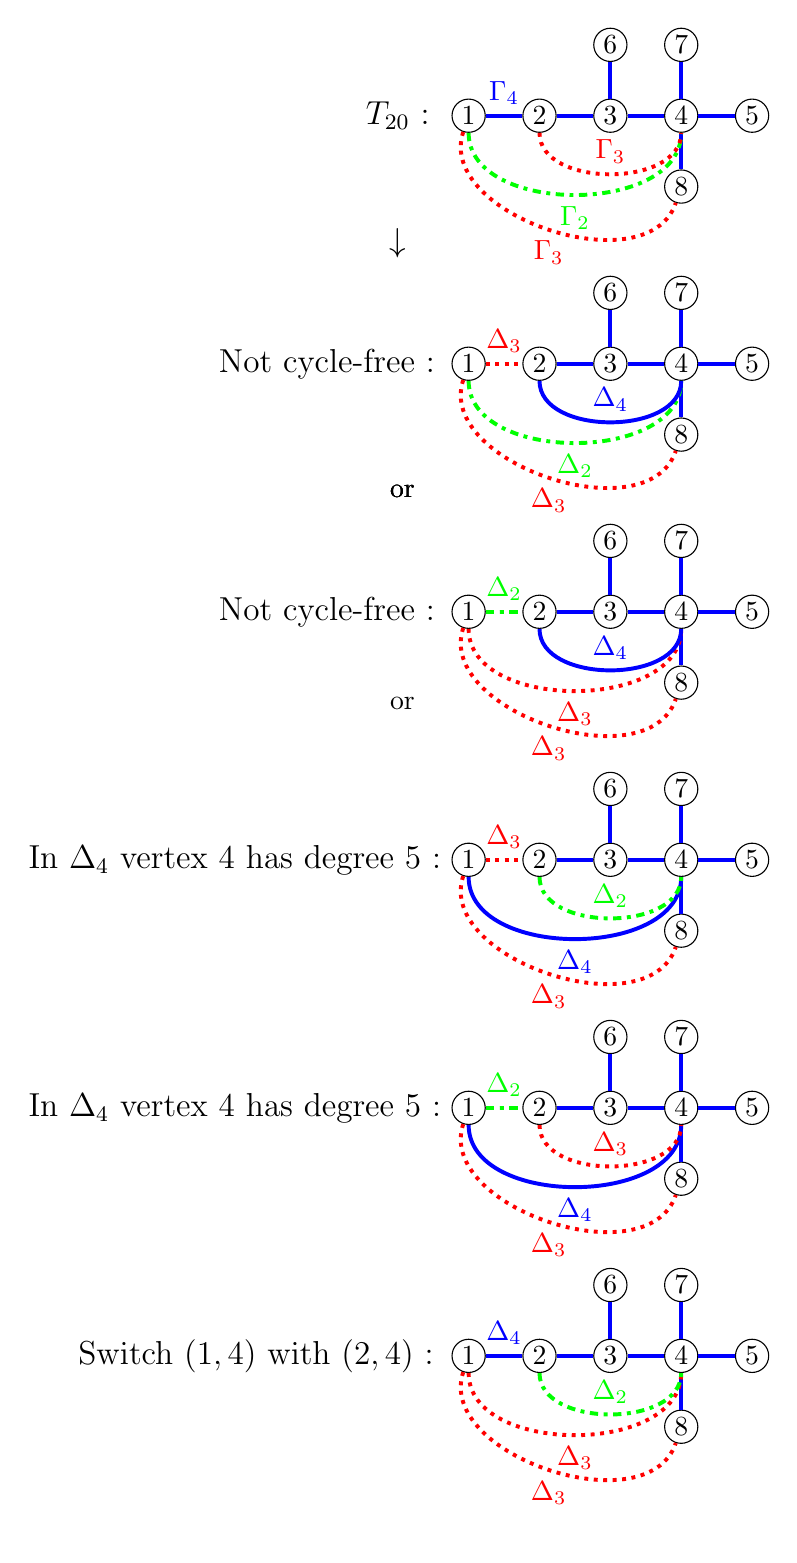
\begin{tikzpicture}
  [scale=0.9,auto=left]%
	
	\node[shape=circle,minimum size = 24pt,inner sep=0.3pt] (m4) at (-1,0) {{\large $T_{20}$ :}};
	\node[shape=circle,draw=black,minimum size = 12pt,inner sep=0.3pt] (n1) at (0,0) {$1$};
	\node[shape=circle,draw=black,minimum size = 12pt,inner sep=0.3pt] (n2) at (1,0) {$2$};
	\node[shape=circle,draw=black,minimum size = 12pt,inner sep=0.3pt] (n3) at (2,0) {$3$};
  \node[shape=circle,draw=black,minimum size = 12pt,inner sep=0.3pt] (n4) at (3,0) {$4$};
	\node[shape=circle,draw=black,minimum size = 12pt,inner sep=0.3pt] (n5) at (4,0) {$5$};
  \node[shape=circle,draw=black,minimum size = 12pt,inner sep=0.3pt] (n6) at (2,1) {$6$};
	\node[shape=circle,draw=black,minimum size = 12pt,inner sep=0.3pt] (n7) at (3,1) {$7$};
  \node[shape=circle,draw=black,minimum size = 12pt,inner sep=0.3pt] (n8) at (3,-1) {$8$};

\node[shape=circle,minimum size = 24pt,inner sep=0.3pt] (m4) at (-1,-1.8) {{\large $\downarrow$}};
\path[line width=0.5mm,blue] (n1) edge[bend left=0] node [above] {$\Gamma_4$} (n2);
\path[line width=0.5mm,blue] (n2) edge[bend left=0] node [above] {} (n3);
\path[line width=0.5mm,blue] (n3) edge[bend left=0] node [above] {} (n4);
\path[line width=0.5mm,blue] (n4) edge[bend left=0] node [above] {} (n5);
\path[line width=0.5mm,blue] (n3) edge[bend left=0] node [above] {} (n6);
\path[line width=0.5mm,blue] (n4) edge[bend left=0] node [below] {} (n7);
\path[line width=0.5mm,blue] (n4) edge[bend left=0] node [above] {} (n8);
\path[line width=0.5mm,green,dash dot] (n1) edge[bend right=90] node [below] {$\Gamma_2$} (n4);
\path[line width=0.5mm,red,dotted] (n2) edge[bend right=90] node [above] {$\Gamma_3$} (n4);
\path[line width=0.5mm,red,dotted] (n1) edge[bend right=90] node [below] {$\Gamma_3$} (n8);

	\node[shape=circle,minimum size = 24pt,inner sep=0.3pt] (m41) at (-2,-3.5) {{\large Not cycle-free :}};
	\node[shape=circle,draw=black,minimum size = 12pt,inner sep=0.3pt] (n11) at (0,-3.5) {$1$};
	\node[shape=circle,draw=black,minimum size = 12pt,inner sep=0.3pt] (n21) at (1,-3.5) {$2$};
	\node[shape=circle,draw=black,minimum size = 12pt,inner sep=0.3pt] (n31) at (2,-3.5) {$3$};
  \node[shape=circle,draw=black,minimum size = 12pt,inner sep=0.3pt] (n41) at (3,-3.5) {$4$};
	\node[shape=circle,draw=black,minimum size = 12pt,inner sep=0.3pt] (n51) at (4,-3.5) {$5$};
  \node[shape=circle,draw=black,minimum size = 12pt,inner sep=0.3pt] (n61) at (2,-2.5) {$6$};
	\node[shape=circle,draw=black,minimum size = 12pt,inner sep=0.3pt] (n71) at (3,-2.5) {$7$};
  \node[shape=circle,draw=black,minimum size = 12pt,inner sep=0.3pt] (n81) at (3,-4.5) {$8$};


\path[line width=0.5mm,red,dotted] (n11) edge[bend left=0] node [above] {$\Delta_3$} (n21);
\path[line width=0.5mm,blue] (n21) edge[bend left=0] node [above] {} (n31);
\path[line width=0.5mm,blue] (n31) edge[bend left=0] node [above] {} (n41);
\path[line width=0.5mm,blue] (n41) edge[bend left=0] node [above] {} (n51);
\path[line width=0.5mm,blue] (n31) edge[bend left=0] node [above] {} (n61);
\path[line width=0.5mm,blue] (n41) edge[bend left=0] node [below] {} (n71);
\path[line width=0.5mm,blue] (n41) edge[bend left=0] node [above] {} (n81);
\path[line width=0.5mm,green,dash dot] (n11) edge[bend right=90] node [below] {$\Delta_2$} (n41);
\path[line width=0.5mm,blue] (n21) edge[bend right=90] node [above] {$\Delta_4$} (n41);
\path[line width=0.5mm,red,dotted] (n11) edge[bend right=90] node [below] {$\Delta_3$} (n81);
	
\node[shape=circle,minimum size = 24pt,inner sep=0.3pt] (m42) at (-1,-5.3) {{ or}};

	\node[shape=circle,minimum size = 24pt,inner sep=0.3pt] (m41) at (-2,-7) {{\large Not cycle-free :}};
	\node[shape=circle,draw=black,minimum size = 12pt,inner sep=0.3pt] (n112) at (0,-7) {$1$};
	\node[shape=circle,draw=black,minimum size = 12pt,inner sep=0.3pt] (n212) at (1,-7) {$2$};
	\node[shape=circle,draw=black,minimum size = 12pt,inner sep=0.3pt] (n312) at (2,-7) {$3$};
  \node[shape=circle,draw=black,minimum size = 12pt,inner sep=0.3pt] (n412) at (3,-7) {$4$};
	\node[shape=circle,draw=black,minimum size = 12pt,inner sep=0.3pt] (n512) at (4,-7) {$5$};
  \node[shape=circle,draw=black,minimum size = 12pt,inner sep=0.3pt] (n612) at (2,-6) {$6$};
	\node[shape=circle,draw=black,minimum size = 12pt,inner sep=0.3pt] (n712) at (3,-6) {$7$};
  \node[shape=circle,draw=black,minimum size = 12pt,inner sep=0.3pt] (n812) at (3,-8) {$8$};


\path[line width=0.5mm,green,dash dot] (n112) edge[bend left=0] node [above] {$\Delta_2$} (n212);
\path[line width=0.5mm,blue] (n212) edge[bend left=0] node [above] {} (n312);
\path[line width=0.5mm,blue] (n312) edge[bend left=0] node [above] {} (n412);
\path[line width=0.5mm,blue] (n412) edge[bend left=0] node [above] {} (n512);
\path[line width=0.5mm,blue] (n312) edge[bend left=0] node [above] {} (n612);
\path[line width=0.5mm,blue] (n412) edge[bend left=0] node [below] {} (n712);
\path[line width=0.5mm,blue] (n412) edge[bend left=0] node [above] {} (n812);
\path[line width=0.5mm,red,dotted] (n112) edge[bend right=90] node [below] {$\Delta_3$} (n412);
\path[line width=0.5mm,blue] (n212) edge[bend right=90] node [above] {$\Delta_4$} (n412);
\path[line width=0.5mm,red,dotted] (n112) edge[bend right=90] node [below] {$\Delta_3$} (n812);
	
\node[shape=circle,minimum size = 24pt,inner sep=0.3pt] (m42) at (-1,-8.3) {{ or}};

	\node[shape=circle,minimum size = 24pt,inner sep=0.3pt] (m413) at (-3.3,-10.5) {{\large  In $\Delta_4$ vertex $4$ has degree $5$ :}};
	\node[shape=circle,draw=black,minimum size = 12pt,inner sep=0.3pt] (n113) at (0,-10.5) {$1$};
	\node[shape=circle,draw=black,minimum size = 12pt,inner sep=0.3pt] (n213) at (1,-10.5) {$2$};
	\node[shape=circle,draw=black,minimum size = 12pt,inner sep=0.3pt] (n313) at (2,-10.5) {$3$};
  \node[shape=circle,draw=black,minimum size = 12pt,inner sep=0.3pt] (n413) at (3,-10.5) {$4$};
	\node[shape=circle,draw=black,minimum size = 12pt,inner sep=0.3pt] (n513) at (4,-10.5) {$5$};
  \node[shape=circle,draw=black,minimum size = 12pt,inner sep=0.3pt] (n613) at (2,-9.5) {$6$};
	\node[shape=circle,draw=black,minimum size = 12pt,inner sep=0.3pt] (n713) at (3,-9.5) {$7$};
  \node[shape=circle,draw=black,minimum size = 12pt,inner sep=0.3pt] (n813) at (3,-11.5) {$8$};


\path[line width=0.5mm,red,dotted] (n113) edge[bend left=0] node [above] {$\Delta_3$} (n213);
\path[line width=0.5mm,blue] (n213) edge[bend left=0] node [above] {} (n313);
\path[line width=0.5mm,blue] (n313) edge[bend left=0] node [above] {} (n413);
\path[line width=0.5mm,blue] (n413) edge[bend left=0] node [above] {} (n513);
\path[line width=0.5mm,blue] (n313) edge[bend left=0] node [above] {} (n613);
\path[line width=0.5mm,blue] (n413) edge[bend left=0] node [below] {} (n713);
\path[line width=0.5mm,blue] (n413) edge[bend left=0] node [above] {} (n813);
\path[line width=0.5mm,blue] (n113) edge[bend right=90] node [below] {$\Delta_4$} (n413);
\path[line width=0.5mm,green,dash dot] (n213) edge[bend right=90] node [above] {$\Delta_2$} (n413);
\path[line width=0.5mm,red,dotted] (n113) edge[bend right=90] node [below] {$\Delta_3$} (n813);
	
\node[shape=circle,minimum size = 24pt,inner sep=0.3pt] (m424) at (-1,-5.3) {{ or}};

	\node[shape=circle,minimum size = 24pt,inner sep=0.3pt] (m4134) at (-3.3,-14) {{\large  In $\Delta_4$ vertex $4$ has degree $5$ :}};
	\node[shape=circle,draw=black,minimum size = 12pt,inner sep=0.3pt] (n1134) at (0,-14) {$1$};
	\node[shape=circle,draw=black,minimum size = 12pt,inner sep=0.3pt] (n2134) at (1,-14) {$2$};
	\node[shape=circle,draw=black,minimum size = 12pt,inner sep=0.3pt] (n3134) at (2,-14) {$3$};
  \node[shape=circle,draw=black,minimum size = 12pt,inner sep=0.3pt] (n4134) at (3,-14) {$4$};
	\node[shape=circle,draw=black,minimum size = 12pt,inner sep=0.3pt] (n5134) at (4,-14) {$5$};
  \node[shape=circle,draw=black,minimum size = 12pt,inner sep=0.3pt] (n6134) at (2,-13) {$6$};
	\node[shape=circle,draw=black,minimum size = 12pt,inner sep=0.3pt] (n7134) at (3,-13) {$7$};
  \node[shape=circle,draw=black,minimum size = 12pt,inner sep=0.3pt] (n8134) at (3,-15) {$8$};


\path[line width=0.5mm,green,dash dot] (n1134) edge[bend left=0] node [above] {$\Delta_2$} (n2134);
\path[line width=0.5mm,blue] (n2134) edge[bend left=0] node [above] {} (n3134);
\path[line width=0.5mm,blue] (n3134) edge[bend left=0] node [above] {} (n4134);
\path[line width=0.5mm,blue] (n4134) edge[bend left=0] node [above] {} (n5134);
\path[line width=0.5mm,blue] (n3134) edge[bend left=0] node [above] {} (n6134);
\path[line width=0.5mm,blue] (n4134) edge[bend left=0] node [below] {} (n7134);
\path[line width=0.5mm,blue] (n4134) edge[bend left=0] node [above] {} (n8134);
\path[line width=0.5mm,blue] (n1134) edge[bend right=90] node [below] {$\Delta_4$} (n4134);
\path[line width=0.5mm,red,dotted] (n2134) edge[bend right=90] node [above] {$\Delta_3$} (n4134);
\path[line width=0.5mm,red,dotted] (n1134) edge[bend right=90] node [below] {$\Delta_3$} (n8134);
	
\node[shape=circle,minimum size = 24pt,inner sep=0.3pt] (m42) at (-1,-5.3) {{ or}};

	
	\node[shape=circle,minimum size = 24pt,inner sep=0.3pt] (m46) at (-3,-17.5) {{\large Switch $(1,4)$ with $(2,4)$ :}};
	\node[shape=circle,draw=black,minimum size = 12pt,inner sep=0.3pt] (n16) at (0,-17.5) {$1$};
	\node[shape=circle,draw=black,minimum size = 12pt,inner sep=0.3pt] (n26) at (1,-17.5) {$2$};
	\node[shape=circle,draw=black,minimum size = 12pt,inner sep=0.3pt] (n36) at (2,-17.5) {$3$};
  \node[shape=circle,draw=black,minimum size = 12pt,inner sep=0.3pt] (n46) at (3,-17.5) {$4$};
	\node[shape=circle,draw=black,minimum size = 12pt,inner sep=0.3pt] (n56) at (4,-17.5) {$5$};
  \node[shape=circle,draw=black,minimum size = 12pt,inner sep=0.3pt] (n66) at (2,-16.5) {$6$};
	\node[shape=circle,draw=black,minimum size = 12pt,inner sep=0.3pt] (n76) at (3,-16.5) {$7$};
  \node[shape=circle,draw=black,minimum size = 12pt,inner sep=0.3pt] (n86) at (3,-18.5) {$8$};


\path[line width=0.5mm,blue] (n16) edge[bend left=0] node [above] {$\Delta_4$} (n26);
\path[line width=0.5mm,blue] (n26) edge[bend left=0] node [above] {} (n36);
\path[line width=0.5mm,blue] (n36) edge[bend left=0] node [above] {} (n46);
\path[line width=0.5mm,blue] (n46) edge[bend left=0] node [above] {} (n56);
\path[line width=0.5mm,blue] (n36) edge[bend left=0] node [above] {} (n66);
\path[line width=0.5mm,blue] (n46) edge[bend left=0] node [below] {} (n76);
\path[line width=0.5mm,blue] (n46) edge[bend left=0] node [above] {} (n86);
\path[line width=0.5mm,red,dotted] (n16) edge[bend right=90] node [below] {$\Delta_3$} (n46);
\path[line width=0.5mm,green,dash dot] (n26) edge[bend right=90] node [above] {$\Delta_2$} (n46);
\path[line width=0.5mm,red,dotted] (n16) edge[bend right=90] node [below] {$\Delta_3$} (n86);

\end{tikzpicture}

\end{document}